\documentclass[12pt, titlepage]{article}

\usepackage{fullpage}
\usepackage[round]{natbib}
\usepackage{multirow}
\usepackage{booktabs}
\usepackage{tabularx}
\usepackage{graphicx}
\usepackage{float}
\usepackage{hyperref}
\usepackage{longtable}
\usepackage{ulem}
\hypersetup{
    colorlinks,
    citecolor=blue,
    filecolor=black,
    linkcolor=red,
    urlcolor=blue
}

\input{../../Comments}
\input{../../Common}

\newcounter{acnum}
\newcommand{\actheacnum}{AC\theacnum}
\newcommand{\acref}[1]{AC\ref{#1}}

\newcounter{ucnum}
\newcommand{\uctheucnum}{UC\theucnum}
\newcommand{\uref}[1]{UC\ref{#1}}

\newcounter{mnum}
\newcommand{\mthemnum}{M\themnum}
\newcommand{\mref}[1]{M\ref{#1}}

\begin{document}

\title{Module Guide for \progname{}} 
\author{\authname}
\date{\today}

\maketitle

\pagenumbering{roman}

\section{Revision History}

\begin{tabularx}{\textwidth}{p{3cm}p{2cm}X}
\toprule {\bf Date} & {\bf Version} & {\bf Notes}\\
\midrule
Jan 9, 2025 & 1.1 & Initial Document\\
Jan 17,2025 & 1.2 & Revised Document Incorporating Feedback\\

\bottomrule
\end{tabularx}

\newpage

\section{Reference Material}

This section records information for easy reference.

\subsection{Abbreviations and Acronyms}

\renewcommand{\arraystretch}{1.2}
\begin{tabular}{l l} 
  \toprule		
  \textbf{symbol} & \textbf{description}\\
  \midrule 
  AC & Anticipated Change\\
  DAG & Directed Acyclic Graph \\
  M & Module \\
  MG & Module Guide \\
  OS & Operating System \\
  R & Requirement\\
  SC & Scientific Computing \\
  SRS & Software Requirements Specification\\
  \progname & Explanation of program name\\
  UC & Unlikely Change \\
  JWT & JSON Web Tokens \\
  MFA & Multi-Factor Authentication \\
  UI & User Interface\\
  \bottomrule
\end{tabular}\\

\newpage

\tableofcontents

\listoftables

\listoffigures

\newpage

\pagenumbering{arabic}

\section{Introduction}

Decomposing a system into modules is a commonly accepted approach to developing
software.  A module is a work assignment for a programmer or programming
team~\citep{ParnasEtAl1984}.  We advocate a decomposition
based on the principle of information hiding~\citep{Parnas1972a}.  This
principle supports design for change, because the ``secrets'' that each module
hides represent likely future changes.  Design for change is valuable in SC,
where modifications are frequent, especially during initial development as the
solution space is explored.  

Our design follows the rules layed out by \citet{ParnasEtAl1984}, as follows:
\begin{itemize}
\item System details that are likely to change independently should be the
  secrets of separate modules.
\item Each data structure is implemented in only one module.
\item Any other program that requires information stored in a module's data
  structures must obtain it by calling access programs belonging to that module.
\end{itemize}

After completing the first stage of the design, the Software Requirements
Specification (SRS), the Module Guide (MG) is developed~\citep{ParnasEtAl1984}. The MG
specifies the modular structure of the system and is intended to allow both
designers and maintainers to easily identify the parts of the software.  The
potential readers of this document are as follows:

\begin{itemize}
\item New project members: This document can be a guide for a new project member
  to easily understand the overall structure and quickly find the
  relevant modules they are searching for.
\item Maintainers: The hierarchical structure of the module guide improves the
  maintainers' understanding when they need to make changes to the system. It is
  important for a maintainer to update the relevant sections of the document
  after changes have been made.
\item Designers: Once the module guide has been written, it can be used to
  check for consistency, feasibility, and flexibility. Designers can verify the
  system in various ways, such as consistency among modules, feasibility of the
  decomposition, and flexibility of the design.
\end{itemize}

The rest of the document is organized as follows. Section
\ref{SecChange} lists the anticipated and unlikely changes of the software
requirements. Section \ref{SecMH} summarizes the module decomposition that
was constructed according to the likely changes. Section \ref{SecConnection}
specifies the connections between the software requirements and the
modules. Section \ref{SecMD} gives a detailed description of the
modules. Section \ref{SecTM} includes two traceability matrices. One checks
the completeness of the design against the requirements provided in the SRS. The
other shows the relation between anticipated changes and the modules. Section
\ref{SecUse} describes the use relation between modules.

\section{Anticipated and Unlikely Changes} \label{SecChange}

This section lists possible changes to the system. According to the likeliness
of the change, the possible changes are classified into two
categories. Anticipated changes are listed in Section \ref{SecAchange}, and
unlikely changes are listed in Section \ref{SecUchange}.

\subsection{Anticipated Changes} \label{SecAchange}

Anticipated changes are the source of the information that is to be hidden
inside the modules. Ideally, changing one of the anticipated changes will only
require changing the one module that hides the associated decision. The approach
adapted here is called design for change.

\begin{description}
\item[\refstepcounter{acnum} \actheacnum \label{acLogin}:] The system should support different authentication methods, such as password-based, biometric login etc.
\item[\refstepcounter{acnum} \actheacnum \label{acTransSpeed}:] The transcription module needs to be optimized to enhance the transcription speed from audio data to written text in real-time. 
\item[\refstepcounter{acnum} \actheacnum \label{acPredModules}:] The diagnosis prediction and medicine prediction modules should be updated with the latest medical knowledge based on the new medical research.
\item[\refstepcounter{acnum} \actheacnum \label{acRealTime}:] The system shall enable real-time streaming of audio input to written text to ensure immediate transcription without delays.   
\end{description}

\subsection{Unlikely Changes} \label{SecUchange}

The module design should be as general as possible. However, a general system is
more complex. Sometimes this complexity is not necessary. Fixing some design
decisions at the system architecture stage can simplify the software design. If
these decision should later need to be changed, then many parts of the design
will potentially need to be modified. Hence, it is not intended that these
decisions will be changed.

\begin{description}
\item[\refstepcounter{ucnum} \uctheucnum \label{ucSecure}:] The requirement to secure patient's profile ensures confidentiality will remain a constant priority in the system.
\item[\refstepcounter{ucnum} \uctheucnum \label{ucCompatible}:] The ability of the system to be compatible with the latest versions of different operating systems such as Windows, Linux and macOS will remain a constant requirement.
\item[\refstepcounter{ucnum} \uctheucnum \label{ucnoisefree}:] The requirement to exclude the background noise while using transcription module is unlikely to change for accurately classification of the medical data.
\item[\refstepcounter{ucnum} \uctheucnum \label{uceaseofuse}:] The system's ease of use is anticipated to remain a constant requirement to allow them to focus on patient's care instead of struggling with the technology. 
\end{description}

\section{Module Hierarchy} \label{SecMH}

This section provides an overview of the module design. Modules are summarized in a hierarchy decomposed by secrets in Table \ref{TblMH}. The modules listed below, which are leaves in the hierarchy tree, are the modules that will actually be implemented.

\begin{description}
  \item [\refstepcounter{mnum} \mthemnum \label{mUAM}:] User Authentication Module
  \item [\refstepcounter{mnum} \mthemnum \label{mAVM}:] Administrator View Module
  \item [\refstepcounter{mnum} \mthemnum \label{mPVM}:] Patient View Module
  \item [\refstepcounter{mnum} \mthemnum \label{mAMM}:] Administrator Model Module
  \item [\refstepcounter{mnum} \mthemnum \label{mPMM}:] Patient Model Module
  \item [\refstepcounter{mnum} \mthemnum \label{mBM}:] Broker Module
  \item [\refstepcounter{mnum} \mthemnum \label{mTM}:] Transcription Module
  \item [\refstepcounter{mnum} \mthemnum \label{mCM}:] Classification Module
  \item [\refstepcounter{mnum} \mthemnum \label{mDPM}:] Diagnosis Prediction Module
  \item [\refstepcounter{mnum} \mthemnum \label{mMPM}:] Medicine Prediction Module
  \item [\refstepcounter{mnum} \mthemnum \label{mAAMM}:] Administrator Account Management Module
  \item [\refstepcounter{mnum} \mthemnum \label{mPAMM}:] Patient Account Management Module

\end{description}

\begin{table}[h!]
\centering
\begin{tabular}{p{0.3\textwidth} p{0.6\textwidth}}
\toprule
\textbf{Level 1} & \textbf{Level 2}\\
\midrule
{Hardware-Hiding Module} & None \\
\midrule
\multirow{7}{0.3\textwidth}{Behaviour-Hiding Module} & \mref{mUAM}\\
& \mref{mAVM}\\
& \mref{mPVM}\\
& \mref{mAMM}\\
& \mref{mPMM}\\
& \mref{mBM}\\
& \mref{mAAMM}\\
& \mref{mPAMM}\\
\midrule

\multirow{3}{0.3\textwidth}{Software Decision Module} & \mref{mTM}\\
& \mref{mCM}\\
& \mref{mDPM}\\
& \mref{mMPM}\\
\bottomrule

\end{tabular}
\caption{Module Hierarchy}
\label{TblMH}
\end{table}

\section{Connection Between Requirements and Design} \label{SecConnection}

The design of the system is intended to satisfy the requirements developed in
the SRS. In this stage, the system is decomposed into modules. The connection
between requirements and modules is listed in Table~\ref{TblRT}.

% \wss{The intention of this section is to document decisions that are made
%   ``between'' the requirements and the design.  To satisfy some requirements,
%   design decisions need to be made.  Rather than make these decisions implicit,
%   they are explicitly recorded here.  For instance, if a program has security
%   requirements, a specific design decision may be made to satisfy those
%   requirements with a password.}

\section{Module Decomposition} \label{SecMD}

Modules are decomposed according to the principle of ``information hiding'' proposed by \citet{ParnasEtAl1984}. The \emph{Secrets} field in a module decomposition is a brief statement of the design decision hidden by the module. The \emph{Services} field specifies \emph{what} the module will do without documenting \emph{how} to do it. For each module, a suggestion for the implementing software is given under the \emph{Implemented By} title. If the entry is \emph{OS}, this means that the module is provided by the operating system or by standard programming language libraries.  \emph{\progname{}} means the module will be implemented by the \progname{} software.

Only the leaf modules in the hierarchy have to be implemented. If a dash (\emph{--}) is shown, this means that the module is not a leaf and will not have to be implemented.

\subsection{Hardware Hiding Modules}

\begin{description}
\item[Secrets:]The data structure and algorithm used to implement the virtual hardware.
\item[Services:]Serves as a virtual hardware used by the rest of the system. This module provides the interface between the hardware and the software. So, the system can use it to display outputs or to accept inputs.
\item[Implemented By:] OS
\end{description}

\subsection{Behaviour-Hiding Module}

\begin{description}
\item[Secrets:]The contents of the required behaviours.
\item[Services:]Includes programs that provide externally visible behaviour of the system as specified in the software requirements specification (SRS) documents. This module serves as a communication layer between the hardware-hiding module and the software decision module. The programs in this module will need to change if there are changes in the SRS.
\item[Implemented By:] --
\end{description}

\subsubsection{User Authentication Module (\mref{mUAM})} 

\begin{description}
\item[Secrets:]The implementation details of the authentication mechanism, including secure storage and validation of user credentials, and session management.
\item[Services:]Authenticates users to grant access to the system based on credentials.
\item[Implemented By:]Spring, React
\item[Type of Module:]Abstract Object
\end{description}

\subsubsection{Administrator View Module (\mref{mAVM})}

\begin{description}
\item[Secrets:]UI customization based on the administrative tools and functionality required by healthcare networks.
\item[Services:]Provide healthcare network adminstrators with tools to onboard, update, and remove their network on the system. Provide healthcare network adminstrators with tools to add healthcare professionals under a healthcare network to the system.
\item[Implemented By:]TypeScript, React
\item[Type of Module:]Abstract Object
\end{description}

\subsubsection{Patient View Module (\mref{mPVM})}

\begin{description}
\item[Secrets:]UI customization based on the tools and functionality required by healthcare professionals.
\item[Services:]Provides healthcare professionals with tools to login, create, update, and delete patient records, provide diagnostic suggestions, and medication suggestions.
\item[Implemented By:]TypeScript, React
\item[Type of Module:]Abstract Object
\end{description}

\subsubsection{Adminstrator Model Module (\mref{mAMM})}

\begin{description}
\item[Secrets:]Represents the healthcare network information and characteristics as a data structure.
\item[Services:]Provides a contract of what is stored in the adminstrator account database and displayed on the UI. Any update in healthare network information on the UI can be reflected in the data model and can directly update the corresponding information in the adminstrator account database.
\item[Implemented By:]TypeScript
\item[Type of Module:]Abstract Object
\end{description}

\subsubsection{Patient Model Module (\mref{mPMM})}

\begin{description}
\item[Secrets:]Represents the patient information and characteristics as a data structure. 
\item[Services:]Provides a contract of what is stored in the patient account database and displayed on the UI. Any update in patient information on the UI can be reflected in the data model and can directly update the corresponding information in the patient account database.
\item[Implemented By:]TypeScript
\item[Type of Module:]Abstract Object
\end{description}

\subsubsection{Broker Module (\mref{mBM})}

\begin{description}
\item[Secrets:]The logic for generating and validating OAuth tokens, handling service interaction, as well as handling communication protocols.
\item[Services:]This module provides:
\begin{itemize}
    \item OAuth 2.0-based request authentication and authorization for all requests.
    \item Secure token generation, validation, and renewal. 
    \item Routing requests between services to fulfill use cases.
\end{itemize}
\item[Implemented By:]Spring, OAuth
\item[Type of Module:]Abstract Object
\end{description}

\subsubsection{Administrator Account Management Module (\mref{mAAMM})}

\begin{description}
\item[Secrets:]Database schema for indexing strategies, and data caching mechanisms for efficient storage and retrieval.
\item[Services:]Manages secure storage, retrieval, and updates of data related to healthcare networks and healthcare professionals.
\item[Implemented By:]MongoDB, Spring
\item[Type of Module:]Record
\end{description}

\subsubsection{Patient Account Management Module (\mref{mPAMM})}

\begin{description}
\item[Secrets:]Database schema for indexing strategies, and data caching mechanisms for efficient storage and retrieval.
\item[Services:]Manages secure storage, retrieval, and updates of data related to patient records.
\item[Implemented By:]MongoDB, Spring
\item[Type of Module:]Record
\end{description}


\subsection{Software Decision Module}

\begin{description}
\item[Secrets:]The design decision based on mathematical theorems, physical facts, or programming considerations. The secrets of this module are
  \emph{not} described in the SRS.
\item[Services:]Includes data structure and algorithms used in the system that do not provide direct interaction with the user. 
  % Changes in these modules are more likely to be motivated by a desire to
  % improve performance than by externally imposed changes.
\item[Implemented By:] --
\end{description}


\subsubsection{Transcription Module (\mref{mTM})}

\begin{description}
\item[Secrets:]The algorithm used to convert audio data into written text.
\item[Services:]Accurately converts the audio data from the conversation into written text.   
\item[Implemented By:]Python
\item[Type of Module:]Library
\end{description}

\subsubsection{Classification Module (\mref{mCM})}

\begin{description}
\item[Secrets:]The algorithm used to classify the medical data after the transcription module.
\item[Services:]Accurately classifies the medical data received from the transcription module into relevant categories.
\item[Implemented By:]Python
\item[Type of Module:]Library
\end{description}

\subsubsection{Diagonsis Prediction Module (\mref{mDPM})}

\begin{description}
\item[Secrets:]The algorithms used to predict possible diagnoses.
\item[Services:]Predicts a set of applicable diagnoses for a patient based on patient characteristics, symptoms, and past medical history.
\item[Implemented By:]Python
\item[Type of Module:]Abstract Object
\end{description}

\subsubsection{Medicine Prediction Module (\mref{mMPM})}

\begin{description}
\item[Secrets:]The algorithms used to give possible medicines applicable.
\item[Services:]Predicts a set of applicable medicines for a patient based on patient characteristics, symptoms, and past medical history.
\item[Implemented By:]Python
\item[Type of Module:]Abstract object
\end{description}


\section{Traceability Matrix} \label{SecTM}

This section shows traceability matrices between the modules and the requirements and between the modules and the anticipated changes.

% the table should use mref, the requirements should be named, use something
% like fref
\begin{table}[H]
\centering
\begin{tabular}{p{0.2\textwidth} p{0.6\textwidth}}
\toprule
\textbf{Req.} & \textbf{Modules}\\
\midrule
FR1 & \mref{mUAM}, \mref{mAVM}, \mref{mAMM}, \mref{mBM}, \mref{mAAMM}\\
FR2 & \mref{mUAM}, \mref{mAVM}, \mref{mAMM}, \mref{mBM}, \mref{mAAMM}\\
FR3 & \mref{mUAM}, \mref{mAVM}, \mref{mAMM}, \mref{mBM}, \mref{mAAMM}\\
FR4 & \mref{mUAM}, \mref{mAVM}, \mref{mAMM}, \mref{mBM}, \mref{mAAMM}\\
FR5 & \mref{mUAM}, \mref{mAVM}, \mref{mAMM}, \mref{mBM}, \mref{mAAMM}\\
FR6 & \mref{mUAM}, \mref{mAVM}, \mref{mAMM}, \mref{mBM}, \mref{mAAMM}\\
FR7 & \mref{mUAM}, \mref{mBM}, \mref{mAAMM}\\
FR8 & \mref{mUAM}, \mref{mPVM}, \mref{mPMM}, \mref{mBM}, \mref{mPAMM}\\
FR9 & \mref{mUAM}, \mref{mPVM}, \mref{mPMM}, \mref{mBM}, \mref{mPAMM}\\
FR10 & \mref{mPVM}, \mref{mPMM}, \mref{mBM}, \mref{mPAMM}\\
FR11 & \mref{mPVM}, \mref{mPMM}, \mref{mBM}, \mref{mTM}, \mref{mCM}, \mref{mPAMM}\\
FR12 & \mref{mPVM}, \mref{mPMM}, \mref{mBM}, \mref{mDPM}, \mref{mPAMM}\\
FR13 & \mref{mPVM}, \mref{mPMM}, \mref{mBM}, \mref{mMPM}, \mref{mPAMM}\\
FR14 & \mref{mUAM}, \mref{mAVM}, \mref{mBM}, \mref{mPAMM}\\
\bottomrule
\end{tabular}
\caption{Trace Between Functional Requirements and Modules}
\label{TblRT}
\end{table}

\begin{table}[H]
\centering
\begin{tabular}{p{0.2\textwidth} p{0.6\textwidth}}
\toprule
\textbf{Req.} & \textbf{Modules}\\
\midrule
NFR1 & \mref{mAVM}, \mref{mPVM}\\
NFR2 & \mref{mAVM}, \mref{mPVM}\\
NFR3 & \mref{mTM}\\
NFR4 & \mref{mAAMM}, \mref{mPAMM}\\
NFR5 & All \\
NFR6 & \mref{mUAM}, \mref{mPAMM}\\
NFR7 & \mref{mPVM}\\
NFR8 & All \\
NFR9 & All \\
\bottomrule
\end{tabular}
\caption{Trace Between Non-Functional Requirements and Modules}
\label{TblRT}
\end{table}


\begin{table}[H]
\centering
\begin{tabular}{p{0.2\textwidth} p{0.6\textwidth}}
\toprule
\textbf{Req.} & \textbf{Modules}\\
\midrule
AC1 & \mref{mBM}\\
AC2 & \mref{mUAM}, \mref{mBM}, \mref{mAVM}, \mref{mAAMM}\\
IR1 & \mref{mUAM}, \mref{mBM}, \mref{mAVM}, \mref{mAAMM}\\
IR2 & All \\
IR3 & \mref{mDPM}, \mref{mMPM}\\
IR4 & \mref{mAAMM}, \mref{mPAMM}\\
IR5 & \mref{mDPM}, \mref{mMPM}\\
IR6 & \mref{mPVM}, \mref{mCM}\\
IR7 & \mref{mPVM}, \mref{mTM}\\
\bottomrule
\end{tabular}
\caption{Trace Between Safety and Security Requirements and Modules}
\label{TblRT}
\end{table}

\begin{table}[H]
\centering
\begin{tabular}{p{0.2\textwidth} p{0.6\textwidth}}
\toprule
\textbf{AC} & \textbf{Modules}\\
\midrule
\acref{acLogin} & \mref{mUAM}\\
\acref{acTransSpeed} & \mref{mTM}\\
\acref{acPredModules} & \mref{mDPM}, \mref{mMPM}\\
\acref{acRealTime} & \mref{mBM}, \mref{mPVM}, \mref{mTM}, \mref{mCM}\\
\bottomrule
\end{tabular}
\caption{Trace Between Anticipated Changes and Modules}
\label{TblACT}
\end{table}

\section{Use Hierarchy Between Modules} \label{SecUse}

In this section, the uses hierarchy between modules is
provided. \citet{Parnas1978} said of two programs A and B that A {\em uses} B if
correct execution of B may be necessary for A to complete the task described in
its specification. That is, A {\em uses} B if there exist situations in which
the correct functioning of A depends upon the availability of a correct
implementation of B.  Figure \ref{FigUH} illustrates the use relation between
the modules. It can be seen that the graph is a directed acyclic graph
(DAG). Each level of the hierarchy offers a testable and usable subset of the
system, and modules in the higher level of the hierarchy are essentially simpler
because they use modules from the lower levels.

% \wss{The uses relation is not a data flow diagram.  In the code there will often
% be an import statement in module A when it directly uses module B.  Module B
% provides the services that module A needs.  The code for module A needs to be
% able to see these services (hence the import statement).  Since the uses
% relation is transitive, there is a use relation without an import, but the
% arrows in the diagram typically correspond to the presence of import statement.}

% \wss{If module A uses module B, the arrow is directed from A to B.}

\begin{figure}[H]
\centering
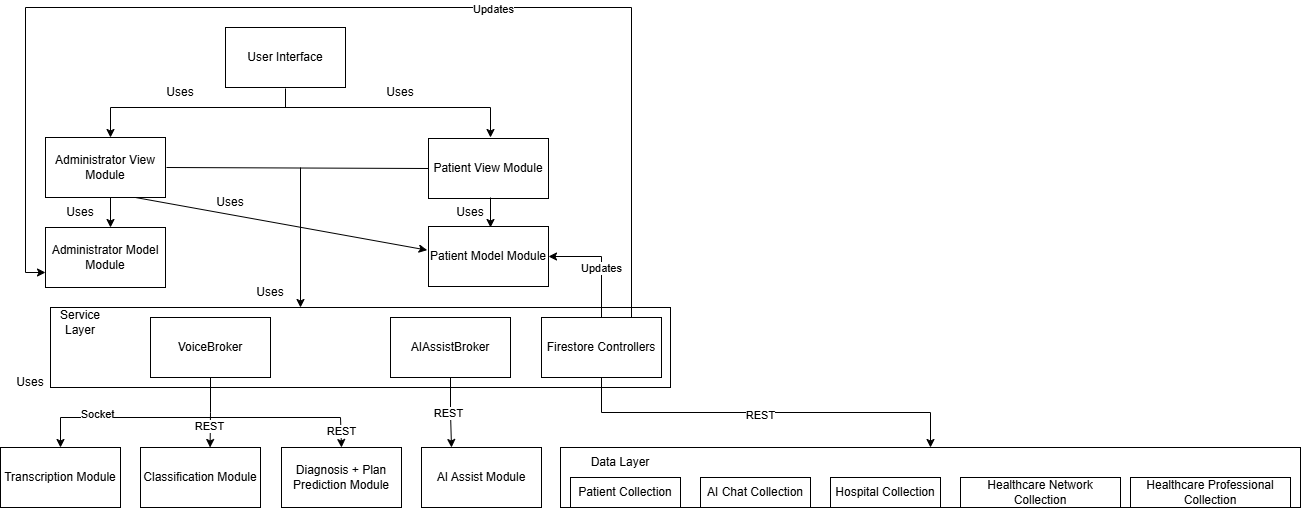
\includegraphics[width=0.7\textwidth]{user-hierarchy.png}
\caption{Use hierarchy among modules}
\label{FigUH}
\end{figure}

%\section*{References}

\section{User Interfaces} \label{sec:UserInterfaces}

The user interfaces for the system are designed to provide an intuitive and efficient user experience for all users, including administrators and healthcare professionals. Below are the key interfaces:


\subsection{Login Interface}
\begin{description}
    \item[Purpose:]Enable users to Login to the system.
   
    \item[Visual Design:]Include input boxes to enter login credentials and signin and signup button to login or create an account respectively.
\end{description}

\begin{figure}[h!]
    \centering
    \fbox{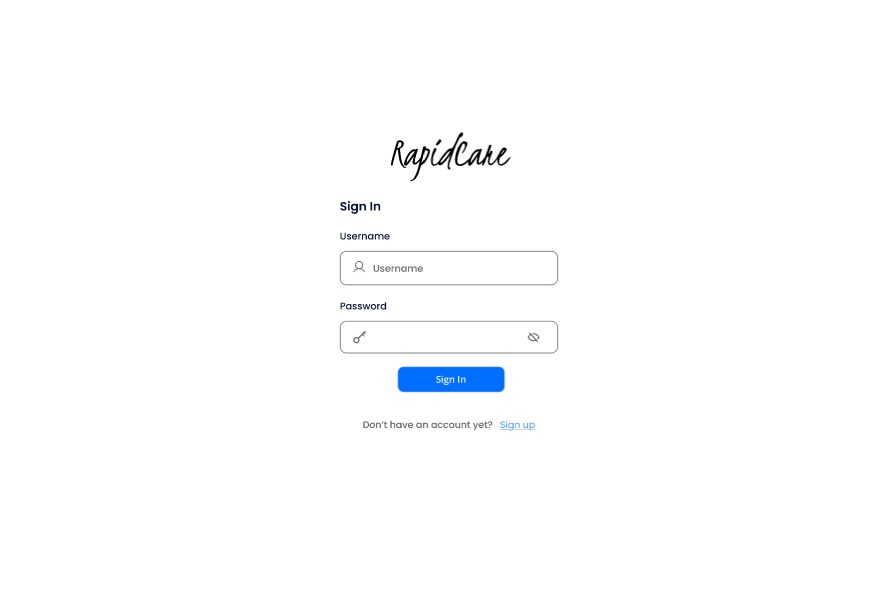
\includegraphics[width=0.8\textwidth,height=6cm]{SignIn.jpg}}
    \caption{Login Interface}
    \label{fig:admin-interface}
\end{figure}

\newpage{}


\subsection{Administrator Dashboard Interface}
\begin{description}
    \item[Purpose:]Enable administrators to manage healthcare network information, view metrics, and manage healthcare professionals.
   
    \item[Visual Design:]Include a navigation bar with options to manage healthcare network, add healthcare professional, reports, and settings. Different menus with an overview of heathcare network metrics.
\end{description}

\begin{figure}[h!]
    \centering
    \fbox{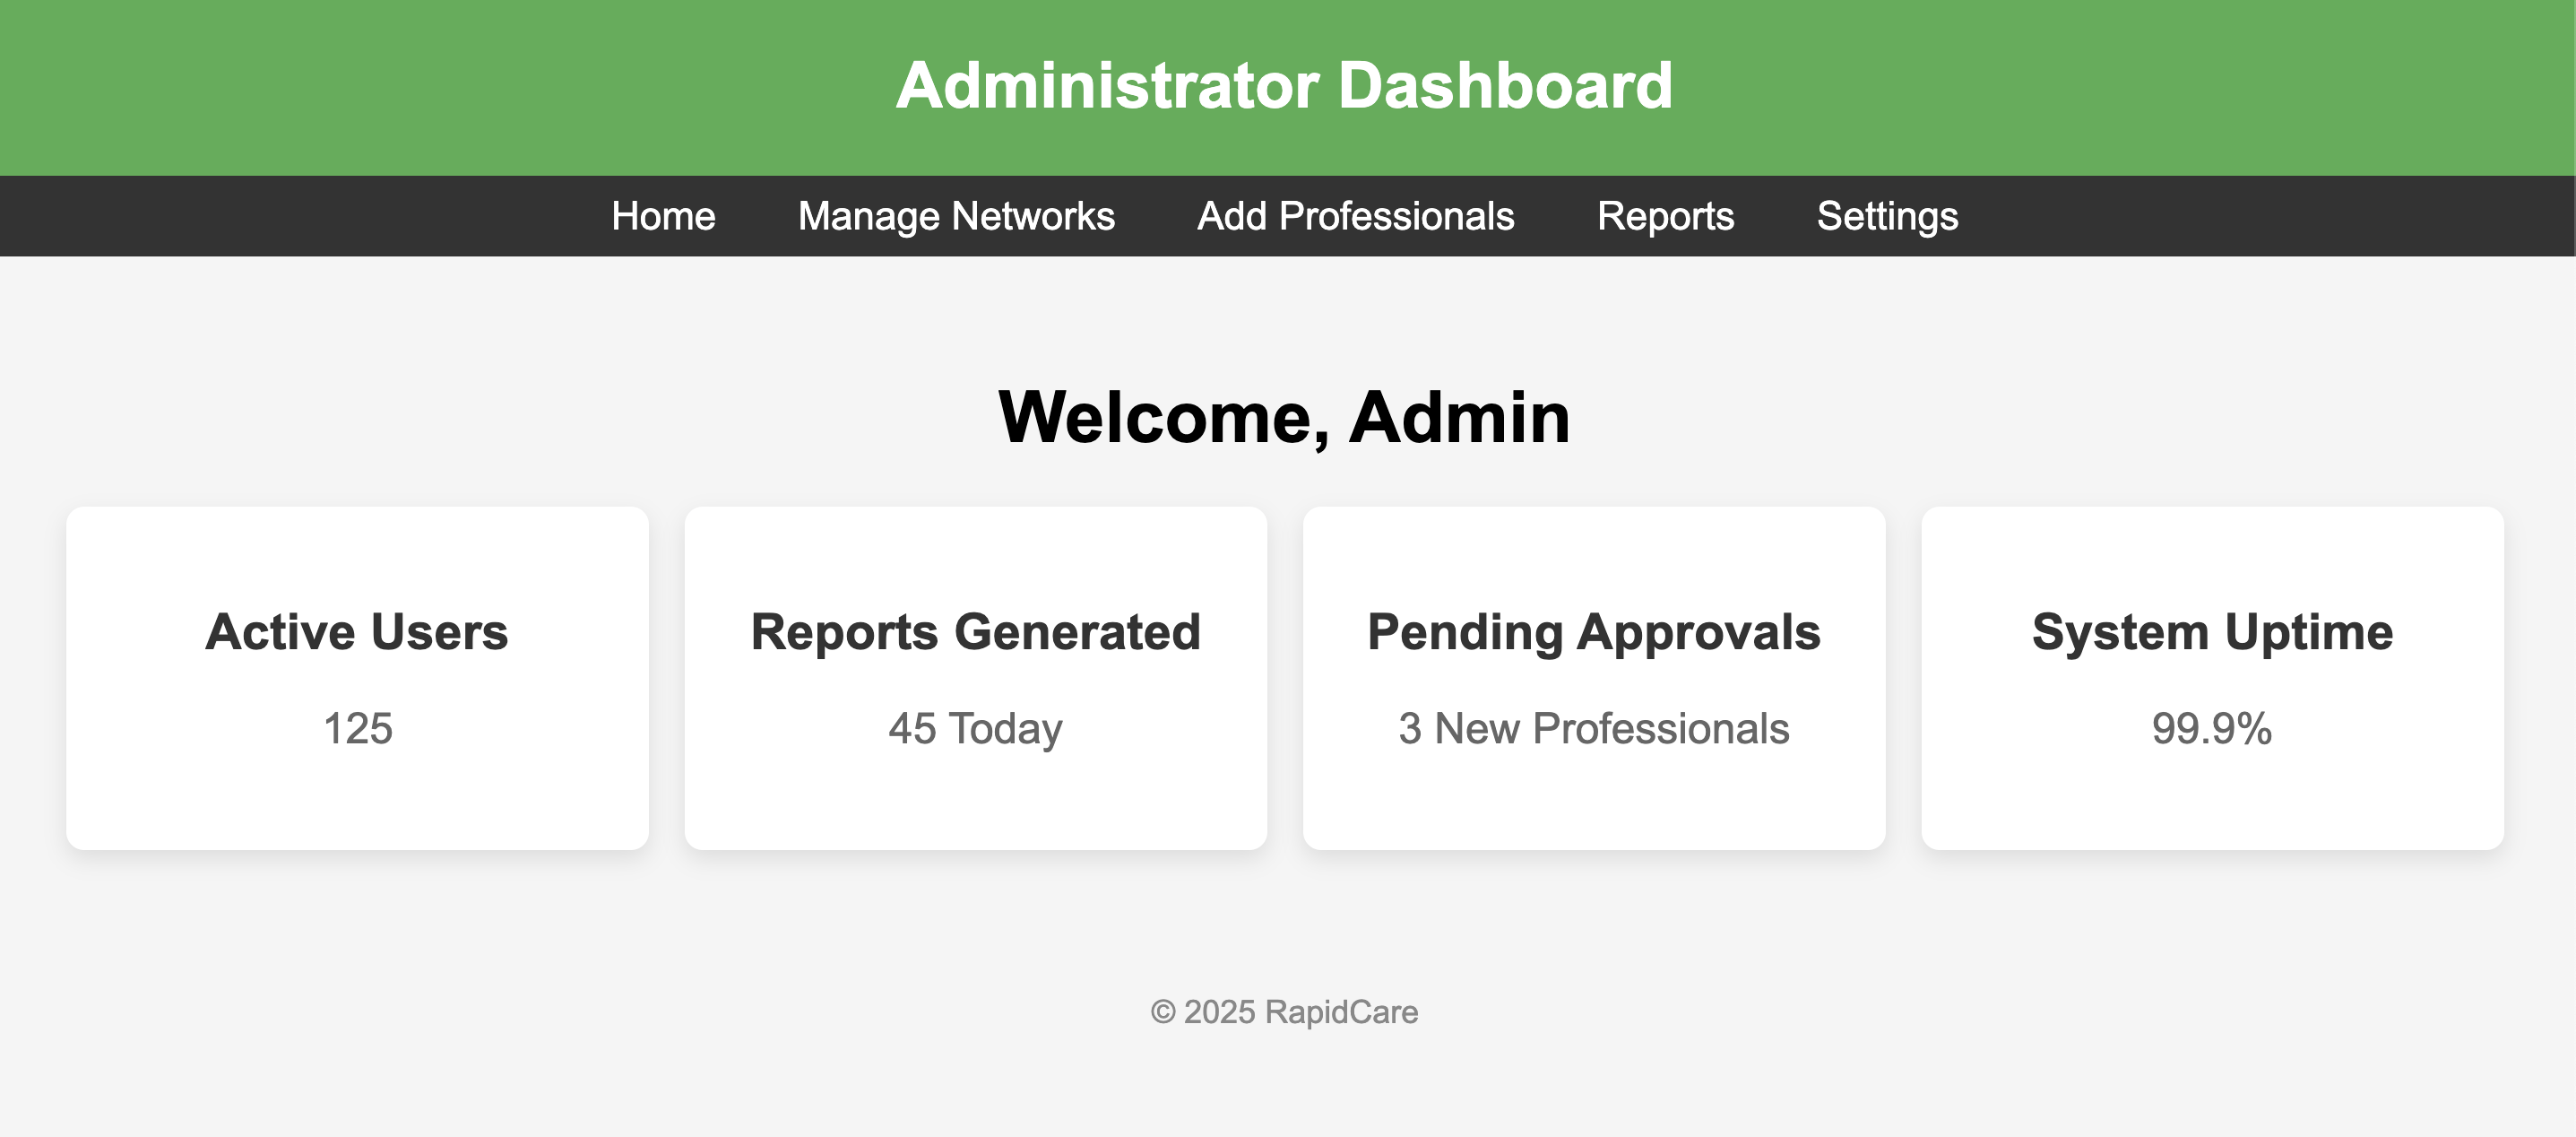
\includegraphics[width=0.8\textwidth,height=6cm]{admin.png}}
    \caption{Administrator Dashboard Interface}
    \label{fig:admin-interface}
\end{figure}

\newpage{}

\subsection{Healthcare Professional Dashboard Interface}
\begin{description}
    \item[Purpose:]Enable healthcare professionals to view metrics, managing patient records, and upcoming appointments.

    \item[Visual Design:]Include a navigation bar with options to view appointments, patient records, notifications, and account information. Different menus with an overview of patient metrics and upcoming appointments.
    
\end{description}

\begin{figure}[h!]
    \centering
    \fbox{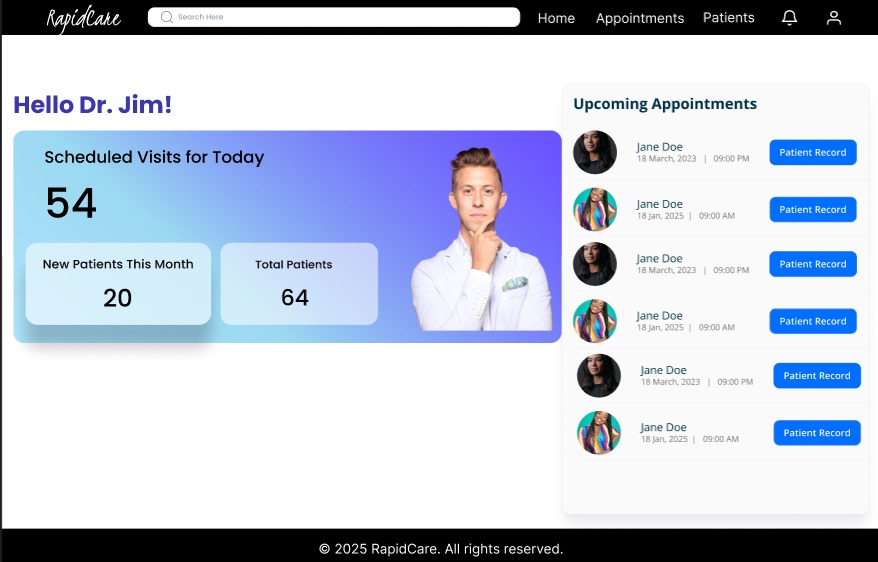
\includegraphics[width=0.8\textwidth,height=6cm]{PatientDashboard.jpg}} 
    \caption{Healthcare Professional Dashboard Interface}
    \label{fig:healthcare-interface-1}
\end{figure}

\newpage{}


\subsection{Patient Profile Interface}
\begin{description}
    \item[Purpose:]Enable healthcare professionals to view and edit patient record.

    \item[Visual Design:]Include a breif overview of the profile and options to edit and close profile. Include a side bar to navigate quickly to frequently used options such as adding a SOAP note, view lab reports etc. Include a navigation bar with options to view profile information, medical history, consultation notes, appointment history, and documents.
    
\end{description}

\begin{figure}[h!]
    \centering
    \fbox{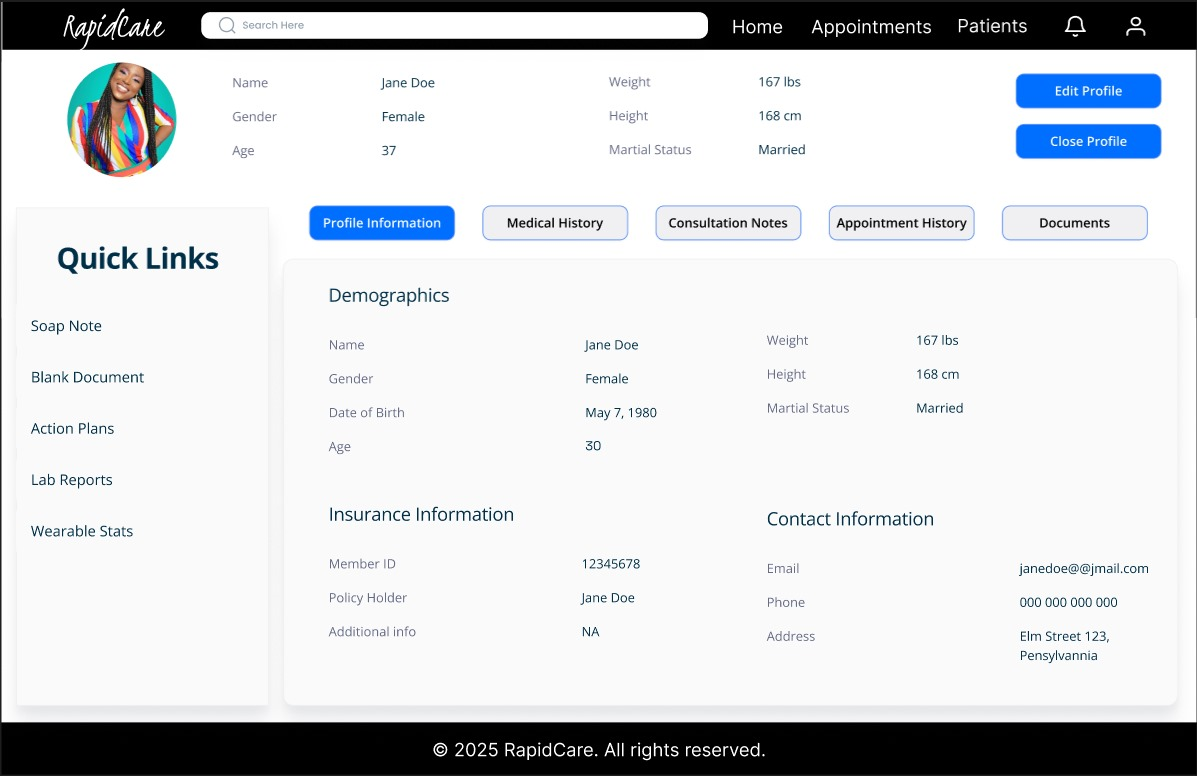
\includegraphics[width=0.8\textwidth,height=6cm]{PatientProfileView.jpg}} 
    \caption{Patient Profile Interface}
    \label{fig:healthcare-interface-2}
\end{figure}

\newpage{}

\subsection{SOAP Note Interface}
\begin{description}
    \item[Purpose:]Enable healthcare professionals add a SOAP note during a consultation and add it to patient profile.

    \item[Visual Design:]Include different fields to add subjective assessment, objective assessment, and assessment summary. Provide different buttons to start recording, stop recording, edit note manually by typing, save note, and go back to profile.
    
\end{description}

\begin{figure}[h!]
    \centering
    \fbox{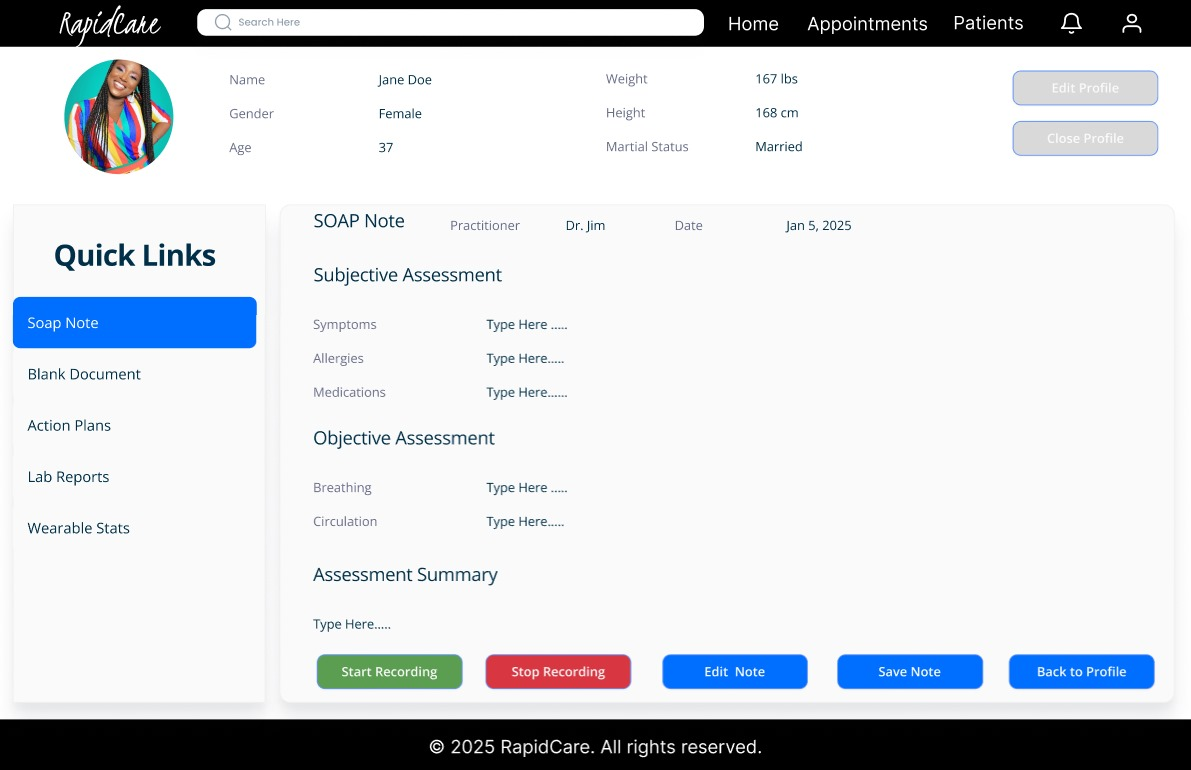
\includegraphics[width=0.8\textwidth,height=6cm]{SOAPView.jpg}} 
    \caption{SOAP Note Interface}
    \label{fig:healthcare-interface-3}
\end{figure}


\section{Design of Communication Protocols}

Due to the broker architectures connecting with various services, the communication protocols differ slightly. For most of the communication as they will be simply `POST` or `GET`. Examples of this communication being used would be fetching patient data from the database, classifying the transcription, or employee retrieval, etc... HTTP communication will be used in \textbf{all} but one use case.

The one use case where HTTP communication will not be used is for the transcription service. For this service we will be using web socket communication as this will provide streaming capabilities for real time transcription. The frontend will act as the client who will send audio chunks to the backend to be transcribed. This will facilitate bidirectional communcation as well.


\section{Timeline}

\begin{itemize}
  \item Week of Jan. 19th -- Rev0 Demonstration:
    \begin{itemize}
      \item Transcription optimization (Gurleen, Pranav)
      \item Text Classification Service Review (Moamen)
      \item Setup Socket communication through API and Transcription Service (Pranav)
      \item Containerize application + Setup deployment environment (Pranav)
      \item Build out login page, dedication classify text UI (Inreet)
    \end{itemize}
  \item Week of Jan. 26th
    \begin{itemize}
      \item Setup ML Training Pipeline (Pranav)
      \item Employee management + Patient Management Views (Inreet, Gurleen)
      \item Data Layer setup (Moamen)
    \end{itemize}
  \item Week of Feb. 2nd
    \begin{itemize}
      \item Rev0 Demonstration
      \item Complete final optimizations and refinements (All)
      \item Worker onboarding FR
    \end{itemize}
  \item Week of Feb. 9th
    \begin{itemize}
      \item Supervisor acceptance meeting + resolve supervisor reviews (All)
    \end{itemize}
  \item Week of Feb. 16th
    \begin{itemize}
      \item VnV Report Completion
      \item Testing introduce testing suites as per VnV.
    \end{itemize}
  \item Week of Feb. 23rd
    \begin{itemize}
      \item VnV Report Completion
    \end{itemize}
  \item Week of Mar. 2nd
    \begin{itemize}
      \item VnV Report Submission
    \end{itemize}
  \item Week of Mar. 9th
    \begin{itemize}
      \item Complete outlying tickets converse with supervisor on additional functionality.
      \item Suggestion model retraining capabilities.
    \end{itemize}
  \item Week of Mar. 16th
    \begin{itemize}
      \item Diagonistic suggestions and Medication suggestions
      \item Usable API for other networks to send patient charts.
      \item Presentation preparation
    \end{itemize}
  \item Week of Mar. 23rd
    \begin{itemize}
      \item Presentation preparation finishing
    \end{itemize}
\end{itemize}

\bibliographystyle {plainnat}
\bibliography{../../../refs/References}

\newpage{}

\end{document}